In this chapter we will briefly discuss the theoretical background used when dealing with two-component coherently coupled spin mixtures of BECs. Since we are dealing with a many-body quantum problem, the standard approach is to use a quantum field to describe the state of the condensate. This leads directly to the Gross-Pitaevskii equation, which will be the starting point of this discussion, after a quick review of the ideal Bose gas. The following content is mostly based on Refs.\ \cite{pitaevskii2016bose} and \cite{lamporesi2023two}.

\section{Ideal Bose gas}
The simplest way to treat the ideal Bose gas (a quantum system of non-interacting bosons) is by relying on the grand-canonical ensemble. 

Let us then recall the probability of the system having a number of particles $N'$ and energy $E_k$ when in contact with a reservoir of temperature $T$ and chemical potential $\mu$:
\begin{equation*}
    P_{N'}(E_k) = e^{\beta(\mu N' - E_k)}\, ,
\end{equation*}
with $\beta = 1/(k_B T)$, from which one can build the \textit{grand-canonical partition function}
\begin{equation}
    \mathcal{Z}(\beta, \mu) = \sum_{N' = 0}^\infty \sum_k P_{N'}(E_k) = \sum_{N' = 0}^\infty e^{\beta \mu N'} Q_{N'}(\beta)\, ,
    \label{eq:part_func}
\end{equation}
where $Q_{N'}$ is the canonical partition function associated to a system of $N'$ (fixed) particles. From the partition function, the physical properties of the system are derived through the calculation of the grand-canonical potential 
\begin{equation}
    \Omega = E - T S - \mu N = -k_B T \log\mathcal{Z}\, .
    \label{eq:GC_potential}
\end{equation}

In the case of a non-interacting system, the total Hamiltonian is $H = \sum_i H_i$, where the single-particle Hamiltonian solves the eigenvalue problem $H_i \phi_i(\mathbf{r}) = \epsilon_i \phi_i(\mathbf{r})$. In this setting, each energy level $\epsilon_i$ is occupied by $n_i$ particles, and thus the total number of particles and the total energy are
\begin{equation*}
    N' = \sum_i n_i\, , \qquad E_k = \sum_i \epsilon_i n_i\, .
\end{equation*}
The partition function of Eq.\ \eqref{eq:part_func} becomes easy to compute, yielding
\begin{equation*}
    \begin{split}
        \mathcal{Z}(\beta, \mu) &= 
        \sum_{n_0 = 0}^\infty \sum_{n_1 = 0}^\infty \cdots\ e^{\beta \mu \sum_i n_i} e^{-\beta \sum_i \epsilon_i n_i} = 
        \left(\sum_{n_0} e^{\beta \mu n_0} e^{-\beta \epsilon_0 n_0}\right)
        \left(\sum_{n_1} e^{\beta \mu n_1} e^{-\beta \epsilon_1 n_1}\right) = \\
        &= \prod_i \sum_{n_i} \left[e^{\beta(\mu -\epsilon_i)}\right]^{n_i} = 
        \prod_i \frac{1}{1-e^{\beta(\mu - \epsilon_i)}}\, .
    \end{split}
\end{equation*}
Note that the condition $\mu < \epsilon_0$ must be satisfied for the convergence of the series. 
It is interesting to study the total number of particles, which can be obtained from the potential of Eq.\ \eqref{eq:GC_potential}:
\begin{equation*}
    N = \langle N' \rangle = -\pdv{\Omega}{\mu} = k_B T \pdv{\log\mathcal{Z}}{\mu} = \sum_i \frac{1}{e^{\beta(\epsilon_i - \mu)}-1} = \sum_i \langle n_i \rangle\, ,
\end{equation*}
hence revealing the famous \textit{Bose-Einstein distribution}
\begin{equation*}
    \langle n_i \rangle = \frac{1}{e^{\beta(\epsilon_i - \mu)}-1}\, .
\end{equation*}
The occupation number of the ground state is $N_0 = \langle n_0 \rangle$ and the remaining particles are called the thermal component $N_T = N - N_0$. 

The origin of the Bose-Einstein condensation phenomenon is that $N_0 \to \infty$ when $\mu \to \epsilon_0$. In particular, at a fixed temperature $T$, the function $N_T(\mu)$ has a maximum $N_c$ at $\mu = \epsilon_0$, while $N_0$ is divergent. This implies that:
\begin{itemize}
    \item if $N_c > N$, then the normalization condition $N = N_0 + N_T$ is satisfied for values of $\mu < \epsilon_0$ and $N_0$ is negligible (no condensation);
    \item if $N_c = N$, it means that we are at the critical temperature $T_c$ defined by $N_T(T = T_c, \mu = \epsilon_0) = N$. Since $N_T$ is an increasing function of $T$, the previous scenario corresponds to $T > T_c$;
    \item if $N_c < N$ (or $T < T_c$), the contribution of $N_0$ is crucial for the normalization and thus the condensation happens.
\end{itemize}
In a finite box of volume $V$, where the lowest energy eigenvalue is $\epsilon_0 = 0$, the condensate fraction for $T < T_c$ is expressed by
\begin{equation*}
    \frac{N_0}{N} = 1-\left(\frac{T}{T_c}\right)^{3/2}\, .
\end{equation*}
Since $N_0 \approx 0$ for $T > T_c$, the function has a discontinuity of its derivative at the critical temperature: a typical symptom of phase transitions.

The behaviour is similar for a system trapped in an external harmonic potential, where the condensate fraction is
\begin{equation*}
    \frac{N_0}{N} = 1-\left(\frac{T}{T_c}\right)^3
\end{equation*}
and the critical temperature depends on the oscillation frequencies.

\section{Gross-Pitaevskii equation}
For a 1D single-component BEC, namely made of only one species of $N$ indistinguishable bosons, one can use a single wavefunction $\psi(x,t)$ to describe its ground state (GS) by exploiting a mean-field approximation, thus revealing the Gross-Pitaevskii equation (GPE):
\begin{equation}
    i\hbar \pdv{\psi(x,t)}{t} = \left[ 
        -\frac{\hbar^2}{2m}\nabla^2 + V(x,t) + g|\psi(x,t)|^2
    \right] \psi(x,t)\, .
\end{equation}
The unusual term in this equation is the one proportional to the square modulus of the wavefunction through the constant $g$, called the \textit{contact interaction constant}, that describes the interactions between bosons. In fact, for an ideal gas of non-interacting bosons, $g = 0$ and one retrieves the standard Schrödinger equation. The interaction constant can be written in terms of the boson-boson scattering length $a$, a typical property of elastic collisions, by
\[
    g = \frac{4\pi\hbar^2}{m}a\, ,
\]
with $g > 0$ for a stable BEC (for $g < 0$ the system is unstable and collapses on itself).

The GPE can be written in its stationary form as
\begin{equation}
    \left[ 
        -\frac{\hbar^2}{2m}\nabla^2 + V(x) + g|\psi(x)|^2
    \right] \psi(x) = \mu \psi(x)\, ,
    \label{eq:GPE_stat}
\end{equation}
where $\mu \approx \pdv{E}{N}$ is the chemical potential and accounts for the energy contribution of a single particle. Spatial properties of the condensate can arise from this equation, especially in the case of $N \gg 1$ and when the interaction term is dominating on the kinetic energy term. By neglecting the kinetic term from Eq.\ \eqref{eq:GPE_stat}, one easily gets the stationary solution
\[
    |\psi(x)|^2 = n(x) = \frac{\mu - V(x)}{g}\, ,
\]
where $n(x)$ is the density distribution, and the association of the latter with the square modulus of the wavefunction leads to the normalization condition $\int |\psi(x)|^2 \dd x = N$. A relevant case is when the external potential is harmonic, yielding a parabolic distribution
\begin{equation}
    n(x) = \frac{\mu - \frac{1}{2}m\omega^2x^2}{g} = 0 \qquad
    \Leftrightarrow \qquad
    x = R_{\rm TF} = \sqrt{\frac{2\mu}{m\omega^2}}\, ,
    \label{eq:TF}
\end{equation}
with $R_{\rm TF}$ being the Thomas-Fermi radius, a parameter indicating the spatial confinement of the condensate.

% Another important property to study is the elementary excitations spectrum due to small perturbations of the GS. It is called the Bogoljubov spectrum and yields
% \begin{equation*}
%     E(k) = \hbar \omega(k) = \sqrt{\frac{\hbar^2 k^2}{2m}\left(\frac{\hbar^2 k^2}{2m} + 2mc^2\right)} \approx
%     \begin{cases}
%         \hbar c k \qquad \text{if} \quad \hbar k \ll mc\\
%         \frac{\hbar^2 k^2}{2m} \qquad \text{if} \quad \hbar k \gg mc
%     \end{cases}\, .
%     \label{eq:excit}
% \end{equation*}

% Also, the healing length is a quantity that expresses how small can spatial changes of the wavefunction be at most. It is
% \begin{equation*}
%     \xi = \frac{1}{\sqrt{8\pi n a}} = \frac{\hbar}{\sqrt{2m n g}}\, .
% \end{equation*}

\section{Two-component mixture}
When the system is composed of two different species ($a$ and $b$), Eq.\ \eqref{eq:GPE_stat} splits into two coupled stationary GPEs:
\begin{equation}
    \begin{aligned}
        &\left[ -\frac{\hbar^2}{2m}\nabla^2 + V(x) + g_{aa}|\psi_a(x)|^2 + g_{ab}|\psi_b(x)|^2
        \right] \psi_a(x) = \mu_a \psi_a(x)\, , \\
        &\left[ -\frac{\hbar^2}{2m}\nabla^2 + V(x) + g_{ab}|\psi_a(x)|^2 + g_{bb}|\psi_b(x)|^2
        \right] \psi_b(x) = \mu_b \psi_b(x)\, .
    \end{aligned}
    \label{eq:GPE_two}
\end{equation}
This is due to the possibility of collisions not only between bosons $a$-$a$ or $b$-$b$, but also of the type $a$-$b$, thus producing three interaction constants $g_{aa}, g_{bb}, g_{ab}$. Depending on those constants' values, the system can assume different behaviours and GS configurations. 

For example, take the case of a flat box potential in a total fixed volume $V$, yielding constant densities. Letting $n_a = |\psi_a|^2$ and $n_b = |\psi_b|^2$, we can express the energy density in the following way:
\begin{equation*}
    \mathcal{E} = \frac{1}{2}g_a n_a^2 + \frac{1}{2}g_b n_b^2 + g_{ab}n_a n_b - \mu_a n_a - \mu_b n_b\, ,
\end{equation*}
where the first three terms represent the interactions between particles of the same type and between different ones, while the last two terms account for the chemical potentials. Now, we state that the system is thermodynamically stable and miscible if and only if the Hessian of $\mathcal{E}$ with respect to $n_a$ and $n_b$ is positive-definite. The calculation is straight-forward:
\begin{equation*}
    H = 
    \begin{bmatrix}
        \pdv[2]{\mathcal{E}}{n_a} &  \pdv{\mathcal{E}}{n_a}{n_b} \\
        \pdv{\mathcal{E}}{n_a}{n_b} &  \pdv[2]{\mathcal{E}}{n_b}
    \end{bmatrix} = 
    \begin{bmatrix}
        g_a &  g_{ab} \\
        g_{ab} &  g_b
    \end{bmatrix} > 0
    \qquad \Leftrightarrow \qquad
    \begin{cases}
        g_a > 0 \\
        g_b > 0 \\
        g_a g_b > g_{ab}^2
    \end{cases}\, .
\end{equation*}
The first two conditions ensure that neither $a$ nor $b$ collapse, while the latter expresses the condition for miscibility. Intuitively, if $g_{ab}$ is small with respect to the other constants, it means that the two species do not interact much one with the other, thus letting themselves mix and spatially overlap. On the other hand, if $g_{ab}$ is big (and positive), they strongly repulse and undergo a phase separation. From now on, only repulsive interactions will be considered, so the only possibilities will be immiscible or miscible (no collapse).

In the more general case of a non-uniform trapping potential, the densities depend from the position and the distributions are correlated with the interaction constants. Considering the harmonic trap and the miscible case, if $g_a > g_b$ then the species $b$ will be confined in a small central region, while the species $a$ will occupy more space.
\begin{figure}[ht!]
    \centering
    \includegraphics[width=0.75\textwidth]{figures/chap1/buoyancy.png}
    \caption{GPE simulation of a two-component balanced mixture in a harmonic potential. The shaded purple region shows the density distribution of population $a$ and the yellow one the population $b$. Here, a small magnetic field is used to break the left-right simmetry. The total density profile is drawn in black. \textit{From Ref. \cite{lamporesi2023two}}.} 
    \label{fig:buoy}
\end{figure}
This is shown in the lower section of Fig.\ \ref{fig:buoy}, while the upper section shows the immiscible case and the buoyancy (again, $g_a > g_b$). One notes that the total density profile is not Thomas-Fermi anymore when $g_a \neq g_b$.

% It is natural to wonder what the excitation spectrum might look like when two components are present, especially when there is spatial overlap between them. The Bogoljubov spectrum of Eq.\ \eqref{eq:excit} is preserved, but now divided into two energy channels, namely spin and density:
% \begin{equation*}
%     E_{d,s}(k) = \hbar \omega_{d,s}(k) = \sqrt{\frac{\hbar^2 k^2}{2m}\left(\frac{\hbar^2 k^2}{2m} + 2mc_{d,s}^2\right)}\, ,
% \end{equation*}
% with the speeds of sound ($+$ for the density and $-$ for the spin) being
% \begin{equation*}
%     c_{d,s}^2 = \frac{(g_a n_a + g_b n_b) \pm \sqrt{(g_a n_a - g_b n_b)^2 + 4g_{ab}^2 n_a n_b}}{2m}\, .
% \end{equation*}
% There are also two distinct healing lengths,
% \begin{equation*}
%     \xi_{d,s} = \frac{\hbar}{\sqrt{2}mc_{d,s}}\, .
% \end{equation*}

\section{Coherently coupled mixture}
When the system is composed of two species of the same atom, such as two hyperfine states, the dynamics become more interesting because of the possible interconversion processes. One possibility is to use a homogeneous microwave radiation, which couples the two internal states $\ket{a}$ and $\ket{b}$, of the type
\begin{equation*}
    \Omega_R(t) \exp{-i\omega_{\rm cpl}t + \phi}\, ,\qquad \text{with }
    \omega_{\rm cpl} = \omega_{ab} + \delta_B\, .
\end{equation*}
Here, $\omega_{ab}$ is the transition frequency between the two coupled states, and in the case of two hyperfine states of the same angular momentum level it includes the linear Zeeman splitting of a small external magnetic field. The coupling frequency $\omega_{\rm cpl}$ differs from $\omega_{ab}$ by a parameter $\delta_B$ called \textit{detuning}.

In this setting, the two-component GPEs of Eq.\ \eqref{eq:GPE_two} become coupled in the following way:
\begin{equation}
    \begin{aligned}
        &\left[ -\frac{\hbar^2}{2m}\nabla^2 + V(x) - \frac{\delta_B}{2} + g_{aa}|\psi_a(x)|^2 + g_{ab}|\psi_b(x)|^2
        \right] \psi_a(x) - \frac{\hbar\Omega_R}{2}\psi_b(x) = \mu_a \psi_a(x)\, , \\
        &\left[ -\frac{\hbar^2}{2m}\nabla^2 + V(x) + \frac{\delta_B}{2} + g_{ab}|\psi_a(x)|^2 + g_{bb}|\psi_b(x)|^2
        \right] \psi_b(x) - \frac{\hbar\Omega_R}{2}\psi_a(x) = \mu_b \psi_b(x)\, .
    \end{aligned}
    \label{eq:GPE_coupled}
\end{equation}
Thanks to this type of coupling, even an immiscible mixture can spatially overlap. In this context, the system can be studied by looking at two distinct energy channels separately, namely the spin $n_a-n_b$ and density $n_a+n_b$. The behaviour of the spin channel is of great interest, because it shows magnetic properties and is what we will focus on. 

In this coupling regime, the wavefunction spatial changes of the condensate have characteristic lengths related to the spin/density channel and the coupling radiation, called \textit{healing lengths}. Here are the spin and the (Rabi) coupling lengths:
\begin{equation}
    \xi_s = \frac{\hbar}{\sqrt{2mn\delta g}}\, ,
    \qquad
    \xi_R = \sqrt{\frac{\hbar}{m\Omega_R}}\, ,
    \label{eq:heal}
\end{equation} 
where $\delta g = (g_{aa}+g_{bb})/2 - g_{ab}$.

\subsection{Ferromagnetism}
The magnetic model of the system is shown in the phase diagram of Fig.\ \ref{fig:ferro}, where a phase transition from \textit{paramagnetism} to \textit{ferromagnetism} occurs.
\begin{figure}[ht!]
    \centering
    \includegraphics[width=0.8\textwidth]{figures/chap1/ferro.png}
    \caption{Phase diagram of the magnetic properties of the system, showing the magnetization of the ground state. When $|\delta g|n < \hbar\Omega_R$ we are in the paramagnetic (PM) region. On the contrary, when $|\delta g|n > \hbar\Omega_R$ the system can be either in the saturated ferromagnetic (SFM) region if $\delta_{\rm eff}$ is large enough or in the ferromagnetic (FM) region. \textit{From Ref. \cite{cominotti2023ferro}}}
    \label{fig:ferro}
\end{figure}
Similarly to the miscible-immiscible phase transition, here the order parameter takes into account the interaction constants, but with the addition of the coupling radiation, and it is the ratio $|\delta g|n/\hbar\Omega_R$, where from now on $n = n(x = 0)$.

The mean-field energy landscape of the system spin channel is given by the asymmetric double well
\begin{equation}
    E_{\rm MF}(Z) = -\hbar\left(|\delta g|n Z^2 + 2\Omega_R \sqrt{1-Z^2} + 2\delta_{\rm eff} Z\right)\, ,
    \label{eq:E_MF}
\end{equation}
where the coupling strength $\Omega_R$ plays the role of the height of the barrier between the wells and the effective detuning $\delta_{\rm eff} = \delta_B + n(g_{aa}-g_{bb})$ contributes to the asymmetry of the wells. Depending on those values, different behaviours may occur. One may set a fixed value for $\Omega_R$ and then probe the magnetic properties by changing $\delta_{\rm eff}$.

\paragraph{Paramagnetism}
In the case of $|\delta g|n < \hbar\Omega_R$, the energy landscape reduces to a single well and thus the system exhibits paramagnetic properties. The magnetization of the ground state changes continously from $Z=-1$ to $Z=1$ and does not depend on the history of the system. 

\paragraph{Ferromagnetism}
On the other hand, when $|\delta g|n > \hbar\Omega_R$ and $|\delta_{\rm eff}| < \delta_{\rm crit}$ to avoid being in the saturated ferromagnetic region,\footnote{As for the paramagnetic case, in the saturated ferromagnetic the energy landscape has only one minimum} the double well creates a metastable state, which can be the ground state depending on the history of the system, yielding an hysteresis cycle and a ferromagnetic behaviour. This will lead directly to the phenomenon of domain walls and bubble formation analyzed in the following section.


\section{False vacuum decay and bubble formation}
False vacuum decay (FVD) is the process of transition between the metastable state and the true ground state of the system (as the lowest in energy). Let us explore the reasons why it happens and how it happens.

\begin{figure}[ht!]
    \centering
    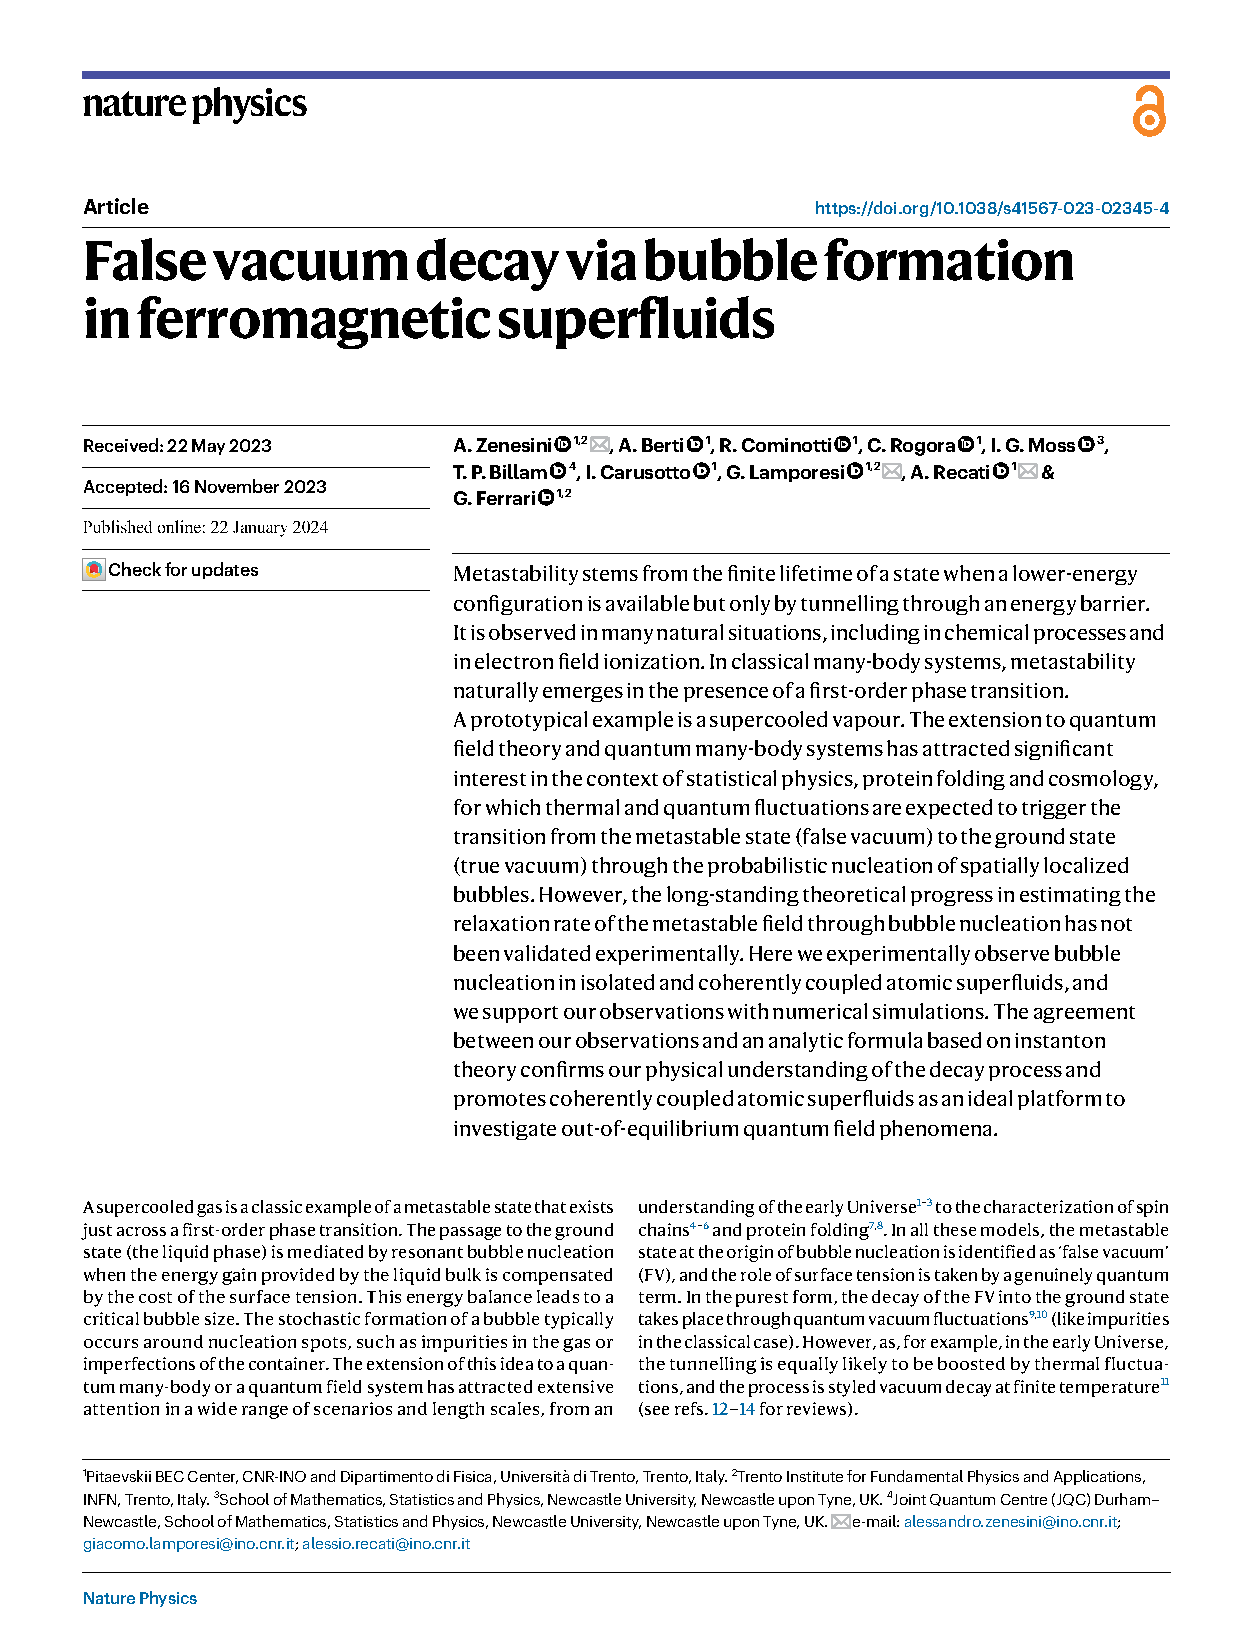
\includegraphics[width=0.5\textwidth]{figures/chap1/FVD.png}
    \caption{Ferromagnetic mean-field energy landscape and false vacuum decay via bubble formation. \textit{From Ref. \cite{zenesini2024false}}.}
    \label{fig:FVD}
\end{figure}

Given the asymmetric double well describing the spin channel mean-field energy landscape of the condensate in the ferromagnetic region (schematic representation in Fig.\ \ref{fig:FVD}), the metastable state A in which all atoms are in the state $\ket{\uparrow}$ is called false vacuum (FV), since it is not the true ground state. The preparation of the system  in this state, as shown in Fig.\ \ref{fig:meta_prep} is not trivial. 
\begin{figure}[ht!]
    \centering
    \includegraphics[width=0.6\textwidth]{figures/chap1/meta_prep.png}
    \caption{Preparation of the system in the metastable FV state by changing the detuning from a positive to a negative value until the energy configuration is the one of Fig.\ \ref{fig:FVD} at $t = 0$. After a waiting time $t > 0$, the system decays into the TV state. \textit{From Ref. \cite{zenesini2024false}}.}
    \label{fig:meta_prep}
\end{figure}
At first, one has to set $\Omega_R$ to a fixed value and $\delta_{\rm eff} > 0$ such that the system is in the saturated ferromagnetic region and the ground state is at positive magnetization. Then, by lowering $\delta_{\rm eff}$, the asymmetry can be shifted until the system is in the metastable state (one must not go beyond $\delta_{\rm eff} = \delta_{\rm crit}$ because it would return to the saturated region). 

The possibility of tunnelling to the state B arises from the fact that the bubble formation has an energy cost due to the kinetic contribution of the interaction on the interface (domain wall) between atoms $\ket{\uparrow}$ and $\ket{\downarrow}$. However, when a sufficient number of atoms in the core region flips to $\ket{\downarrow}$, the energy gain compensates the kinetic cost and the tunnelling can occur resonantly from A to B.\footnote{Pure quantum tunnelling occurs at $T = 0$. At non-zero temperature the processed is helped by thermal excitations.} Once happened, the system is not in a metastable state anymore, hence the decaying into the ground state C, the true vacuum (TV), via bubble expansion with more atoms flipping into the $\ket{\downarrow}$ state. Note that the TV is not composed of all atoms $\ket{\downarrow}$. This is because while the $\ket{\downarrow}$ state is energetically lower in the high-density core region, the situation is opposite in the low-density tails, due to the dependence of the effective detuning on the density.

From an experimental point of view, the parameters to vary are $\Omega_R$ and $\delta_{\rm eff}$, that contribute to the energy landscape and hence to the decay process. However, we expect FVD to be greatly influenced by the depth of the well (the energy difference between FV and TV) and not by the detuning, beacuse the framework where one realizes the experiment is that of $\delta_{\rm eff} \gg \delta_{\rm eff}-\delta_{\rm crit}$, where the tunnelling barrier is shallow.

Another important factor to focus on is time. The reason is that the tunnelling through the energy barrier is a stochastic process and does not happen at a fixed time. The problem arises when one is willing to study the bubble evolution during the decay. After the condensate is prepared in the metastable state, we can wait for an interval of time $\Delta t$ and then decide to look at the system, but due to its quantum nature, a measure will destroy our information, and we will not be able to let it evolve. The system will have to be prepared again in the initial state and so on. By recreating the experiment many times, changing the experimental wating time, one should get a fair picture of the bubble evolution, but relying on time only may not be enough. Since we know the bubble expands, it will be useful to look at its size, $\sigma_B$, as an evolution parameter.



% What is interesting to study is the energy dissipation of the decay during the expansion. The key point is that since the coherent coupling prohibits the system to emit photons, the energy must dissipate through the spin and/or density channel, possibly with waves. Investigating this phenomenon is the purpose of this thesis' data analysis.

